\section{课程简介}

\subsection{学什么}

	\begin{itemize}
		  \item {\bf Wikipedia——微积分} 
		\begin{itemize}
		  \item Latin, {\it a small stone used for counting}  
		  \item {\it a branch of mathematics focused on {\b limits, functions,
		  	derivatives, integrals,}  and {\b infinite series}} 
	  	  \item {\it widespread application in {\b science, economics,} and {\b
	  	  engineering}} 
% 		  \item {\it constitues a major part of modern mathematics} 
		\end{itemize}
		\item {\bf John von Neumann} ({\small\it The Mathematician, 1947})
		\begin{itemize}
		  \item {\it The calculus was the first achievement of modern
		  mathematics, and it is difficult to overestimate its importance.}
		\end{itemize}
		  \item James Stewart, Calculus(5th eds.), 2004
		  \begin{itemize}
		    \item {\it Calculus is fundamentally different from the mathematics that
		    you have studied previously}
		    \item {\it Calculus is less static and more {\b dynamic}}
		    \item {\it It is concerned with change and {\b motion}}
		    \item {\it It deals with quantities that {\b approach} other
		    quantities}%\marginpar{note}
		  \end{itemize}
		\end{itemize}

	\begin{center}
		\scalebox{0.3}{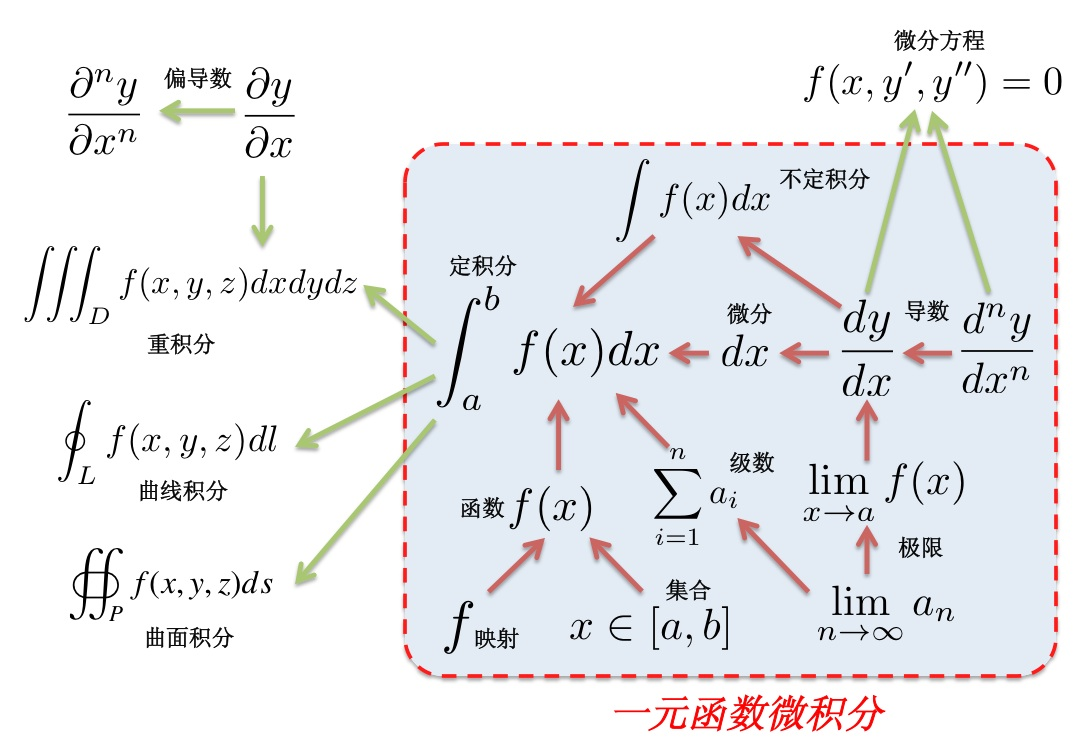
\includegraphics{./images/ch1/AM_architecture.jpg}}
	\end{center}

\subsection{怎么学}
	
\begin{itemize}
	\item {\bf 参考资料}
  	\begin{enumerate}
		\item {\bf 课程配套辅导}
	  	\begin{itemize}
	    	\item {李建平 等,高等数学典型例题与解法(上、下),国防科技大学出版社,2009,长沙} 
	  	\end{itemize}
  		\item {\bf 参考书} 
  		\begin{itemize}
	    	\item {\b 同济大学数学系,高等数学(第六版,上、下),高等教育出版社,2006,北京} 
	    	\item 菲赫金哥尔茨,微积分学教程(第一至三卷),第8版,高等教育出版社,2006,北京 
	    	\item James Stewart, Calculus(5th eds.)(影印版,上、下册),高等教育出版社,2004,北京
	    	\item 任何有关教学内容和{\b 数学历史}的书籍
  		\end{itemize}
	\end{enumerate}
	  \item {\bf 学习方法}
	\begin{itemize}
	  		\item {\bf 听课}\dotfill {\bb 30}
		\begin{itemize}
	  		  \item 典型问题、典型方法
	    	  \item 师傅领进门,修行在个人
	 	\end{itemize}
	  		\item {\bf 练习}\dotfill {\bb 50}
	 	\begin{itemize}
	    		\item 熟能生巧!
	    		\item 记忆!琢磨!
	  	\end{itemize}
	  		\item {\bf 思考}\dotfill {\bb 20}
	  	\begin{itemize}
	    		\item 总结!
	    		\item 质疑!
	  	\end{itemize}
	\end{itemize}
\end{itemize}

\section{几点要求}
\begin{itemize}
	\item {\bf 课堂:安静!安静!!安静!!!}
	
	{\bf - No to}
	  \begin{itemize}
	    \item Chatting
	    \item zZZ\ldots
	    \item anything noisy
	    \item \ldots
	  \end{itemize}
	{\bf - Yes to}
  \begin{itemize}
    \item listen to me
    \item discuss {\bf with me}
    \item do sth. you like {\bf quietly}
    \item zzz\ldots
    \item leave/enter the classroom {\bf quietly}
    \item \ldots
  \end{itemize}
  \item {\bf 作业}
  \begin{itemize}
    \item 正确、规范、工整
    \item no copy !!!!
    \item 订正每一个错误!
  \end{itemize}
	\item {\bf 答疑}
	  \begin{itemize}
	    \item 有问必答
	    \item 除了问考试、问隐私
	  \end{itemize}
% 	  \item {\bf 从善如流}
\end{itemize}

\chapter{映射与函数}

{\bf 关键词:}集合、集合论、映射、函数、曲线及其表示

\section{集合与映射}

\subsection{集合}

{\it Cantor,1874:}\ps{对于集合,“我们只需描述它,而不必给出精确的定义”}
所谓{\b 集合},是指把一些个体({\b 元素}) 放在一起考虑时它们形成的整体。
\begin{itemize}
  \item 关系符号:$\subset, \in, =, \subseteq, \neq$
  \item 运算符号:$\cap,\cup, \setminus, \bar{A}, \times, +, - $
\end{itemize}
	
{\bf 常见(用)的集合:}
$\mathbb{N}\subset\mathbb{Z}\subset\mathbb{Q}\subset\mathbb{R}\subset\mathbb{C}$
\ps{本书约定,自然数集包含数$0$}
	
{\bf 注:}通过集合的笛卡尔乘积{\b “$\times$”} 可以定义更{\bf “高维”}的集合,例如:\\
	\centerline{$\mathbb{R}^2=\mathbb{R}\times\mathbb{R}$}

\subsection{区间和领域}

{\bf 例:}$(a,b)=\{x|a<x<b\}=\{x\in\mathbb{R}|a<x<b\},a,b\in\mathbb{R}$

{\bf 例:}$\mathbb{R}=(+\infty,-\infty)$

{\bf 注意:}$\pm\infty$都不是一个具体的数,因此不能写
$$x=+\infty,\quad x=-\infty$$
而只有
$$x\to+\infty,\quad x\to\infty$$

{\bf 领域:}“与$a$邻近,距离不超过$\delta$”
$$U(a,\delta)=(a-\delta,a+\delta)=\{x||x-a|<\delta\}$$

{\bf 例:}
$$(a,b)=\left(\df{a+b}2,\df{b-a}2\right)$$

{\bf 去心邻域}
$$U_0(a,\delta)=(a-\delta,a+\delta)-\{a\}=\{x|0<|x-a|<\delta\}$$

{\bf 无穷邻域}
$$\{x||x|>M\},\;M>0$$

{\bf 问:}可以写成$U(\infty,M)$吗?

{\bf 注:}类似地,可以有所谓的半邻域,左(右)领域

\begin{shaded}

{\bf 集合论、Russell Paradox与公理系统}

	{\it Cantor,1874:}朴素集合论的诞生。	

	{\it Poincare,1900,国际数学家大会:} 
		 {“\ldots 借助集合论概念,我们可以建造整个数学大厦\ldots  今天,我们可以说绝对的严格性已经达到了\ldots”}
	
	{\it Russell, 1901:}只给不给自己理发的人理发的理发师该不该给自己理发?
	
	“由所有不包含集合自身的集合所构成的集合”,记为$S$。不论$S$是不是自身的元素,按照$S$的定义都会有矛盾。
	
	设$x\in A$表示:$A$给$x$理发, 定义
	$$A=\{x|x\notin x\},$$ 
	
	问:$A\in A$还是$A\notin A$? 
	
% 	\ba{罗素悖论导致了第三次“数学危机”的出现!}
	{{\bf {第三次“数学危机”}}(Frege,1901,《算术基础》)}
		“在工作结束之后发现那大厦的基础已经动摇,对于一个科学工作者来说,没有比这更不幸的了”
		
	\begin{itemize}
	  \item {{\bf 无限抽象原则}(Cantor,Frege):} 任意给定某个条件就可以确定一个集合。(每个概念的外延可以确定一个集合)
	  \item {\bf 观点:}不加限制地使用无限抽象原则将导致罗素悖论
	  \item {{\bf 有限抽象原则}(限制公理):} 如果已知一个集合和一个给定的条件,则该集合中所有满足条件的元素{\b 可以}构成一个集合。
	  \item {\bf ZFS(Zermelo-Fraenkel-Skolem)公理化集合系统}
	  
	  {\bf 命题:}在ZFS中,无法定义包含所有集合的集合。
	
	{\bf 证明:}反证法。设$A$是一个这样的集合。定义
	$$B=\{x\in A|x\notin x\}$$
	若
	$B\in A$,则必有$B\in B$或$B\notin B$。而若$B\in B$,可推出$B\notin B$;同理,
	由$B\notin B$,也可推出$B\in B$。从而$B\notin A$,推出矛盾。这说明$B$的定义存在问题,故知假设错误。

	\item {\bf 公理(Axiom):}无须证明即为正确的命题。
	\begin{itemize}
	  \item {\bf Engles:}数学上的所谓公理,是数学需要用作自己出发点的少数思想上的规定 
	  \item {\bf ZFS系统:}公理就是一些关于逻辑符号{“$\in$”}和{字母}的组合使用方法的约定
	  \item {\bf 公理化方法}是构建现代数学理论体系的基石
	\end{itemize}
	\item {\bf {数学等于永恒的真理吗?}}
	\end{itemize}
\end{shaded}
	
\subsection{实数集的性质}
	\begin{enumerate} 
	  \item {\bf 有序性}($\mathbb{R}^2$、$\mathbb{C}$不具备有序性) 
	  \item {\bf 完备性(连续性): }实数集与数轴上的点之间存在一一对应
	  
	  {\bf{连续性公理(确界原理):}}非空有{\b 上界}的实数集必有{\b 上确界} (最小的上界)
	\end{enumerate}
	
	{\bf 注:}有理数集不满足连续性公理。
	
	{\bf 例:$e=\mathrm{sup}\left\{\left(1+\frac
	1n\right)^n\right|n\in\mathbb{N}\}\notin\mathbb{Q}$}
	\begin{center}
		\resizebox{!}{5cm}{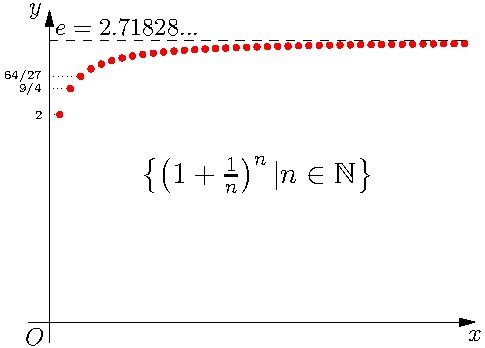
\includegraphics{./images/ch1/e-notin-N.pdf}}
% 		\resizebox{!}{4.8cm}{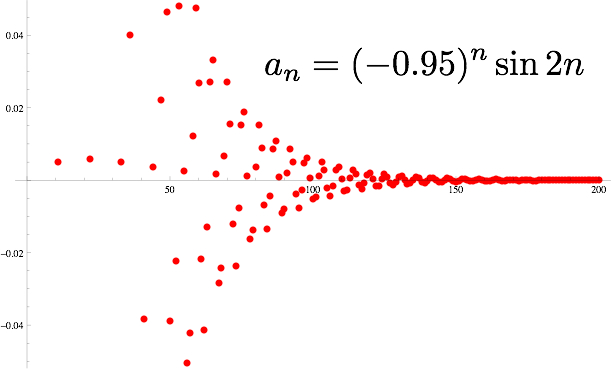
\includegraphics{./images/ch2/sin2nn.jpg}}
% 		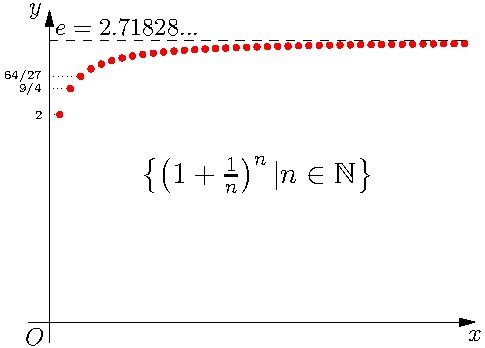
\includegraphics[width=6cm]{./images/ch1/e-notin-N}
	\end{center}
	$$\left(1+\frac11\right)^1<\left(1+\frac12\right)^2<\left(1+\frac13\right)^3<\ldots
	\left(1+\frac1n\right)^n<\ldots<e$$
	
	{\bf 思考:}上确界和最大值有什么异同?如何确定一个集合的上确界?

\subsection{映射}

{\bf 教材P7:}事物之间“一对一”或“多对一”的依赖关系\ps{映射结果必须是无歧义的!}

$$f:A\to B$$
或
$$y=f(x),\;x\in A,y\in B$$

{\bf 三要素:}定义域、值域、对应关系,任何一项不明确都不足以确定一个函数
\ps{有时候只有定义域和对应关系亦可,前提是默认假设映射为满射}

{{\bf 例:}以下函数中哪些是完全相同的?}
		$$x,\quad |x|,\quad e^{\ln x},\quad \ln(e^x),\quad \sqrt{x^2},\quad
		\frac{x^2-4}{x-2}-2,$$
		$$\sin(\arcsin x),\quad \arcsin(\sin x), \quad \tan(\arctan x)$$

{\bf 相关概念:}单射、满射、一一映射(双射)

\begin{shaded}
	{\bf 一一映射与无穷集合}
	
{\bf 问题:}如何比较两个集合中元素的个数?
\begin{itemize}
  \item 自然数与正偶数一样多?({$\surd$})
  \item 自然数与整数一样多?({$\surd$})
  \item 自然数与有理数一样多?({$\surd$})
  \item 区间$(a,b)$中的实数与$\mathbb{R}$中一样多?({$\surd$})
  \item 自然数与实数一样多?({$\times$})
\end{itemize}
	
{\bf 无穷集合:}可以和自身的某个子集建立起一一映射的集合
\end{shaded}	

	
\section{函数}
	
	\begin{shaded}
		{\bf 关于函数}
		\begin{itemize}
		  \item 微积分是关于运动和变化的数学;
		  \item 函数是对运动(例如:曲线、曲面、波以及各种变化)变化过程中各种量与量的依赖关系的抽象描述;
		  \item 函数刻画了运动变化中的量之间的相互依存关系({\bf 注:}与“依存”对应的关系叫做“独立”)
		\end{itemize}
		
		{\bf 常量和变量}
		\begin{itemize}
		  \item {\bf 常量和变量是相对的},在一定条件下可以相互转化
		  \item 变量之间的关系可能是相互依存,也可能是相互独立的
		  \item 为了避免讨论过于复杂,简化问题,我们可能选择只考虑部分参数的变化,而将其他参数视为(或设为)常量,
		  例如:万有引力与两个物体的质量、距离以及引力常数(系数)都有关,为了确定其数量关系,需要事先假定部分的参数
		  值是固定不变的
		\end{itemize}
		
		{\bf 大学数学与中学数学}
		\begin{itemize}
		  \item 数学并无严格的“高等”和“初等”之分,只是存在众多的分支和领域
		  (例如:代数、几何、分析、图论,几何又分为平面几何、立体几何、解析几何等),
		  不同分支或领域的直观性和难度各有不同
		  \item 对于函数,中学阶段更注重在对应关系“确定”的情况下,寻找其数学描述或利用给定的值进行计算
		  \item 大学阶段,从微积分开始,更着重对函数的整体特性,以及不同函数间的转换、类比和关于其整体特征的计算与分析
		\end{itemize}
	\end{shaded}

	{\bf (一元)函数:}由实数集到实数集的映射
	$$f:D\to\mathbb{R},\;(D\subset\mathbb{R})$$
	或
	$$y=f(x),\;(x\in D\subset\mathbb{R},y\in\mathbb{R})$$
% 	\begin{itemize}
% 	  \item {\bf 定义域:} $D\subset \mathbb{R}$ ,且$D\ne\phi$ 
% 	  \item {\bf 对应关系:} $f:D\to\mathbb{R}$
% 	\end{itemize} 
	{\bf 函数图像}
	$$G_f=\{(x,f(x))|x\in D_f\}$$
	
	\begin{shaded}
		{\bf 多元函数:} 
		$$f:D\to\mathbb{R},\quad D\in\mathbb{R}^n$$
		
		{\bf 向量值函数:}
		$$f:D\to\mathbb{R}^,\quad, D\in\mathbb{R}$$
		
		{\bf 思考:}二元函数和三维的向量值函数对应的几何对象分别是什么?
		
		{\bf 思考:}平面曲线与一元函数具有一一对应关系吗?空间曲面和二元函数呢? (No)	
	\end{shaded}	
		\begin{center}
			\resizebox{!}{4.2cm}{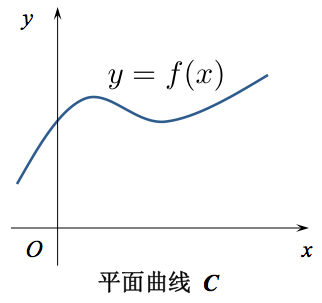
\includegraphics{./images/ch1/C_fx.jpg}}\quad	
			\resizebox{!}{4.5cm}{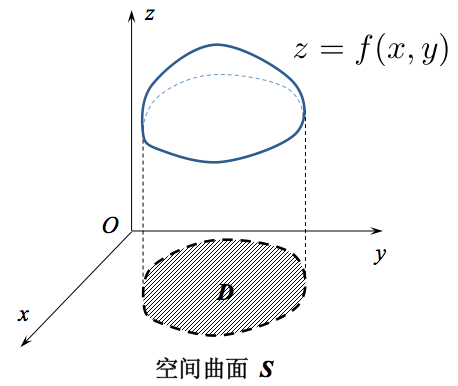
\includegraphics{./images/ch1/S_fxy.jpg}}
		\end{center}
	
\subsection{函数的运算与简单性质}

{\bf 运算:}四则运算、复合运算、逆运算	
	
\begin{shaded}
{\bf 常用数学符号}
	\begin{itemize}
	  \item {\b$\bm{\forall}$} \quad 任意 (for all)
	  \item {\b$\bm{\exists}$} \quad 存在 (exist)
	  \item {\b$\bm{\Rightarrow}$} \quad 推出 (deduce, imply)
	  \item {\b$\bm{\Leftrightarrow}$} \quad 等价 (equivalent, if and only if)
	  \item {\b$\bm{\to}$} \quad 趋于 (approach)
	\end{itemize}
\end{shaded}

\subsubsection{【有界性】}			

{{\bf 定义:}}
	设$I\subset\mathbb{R}$,$f(x)$在$I$上有定义,若集合
	$$\{f(x)|x\in I\}$$
	有界,则称{\bf $f(x)$在$I$上有界}或{\bf $f(x)$是$I$上的有界函数}
		
	{\bf 注:}函数的有界性等价于其值域的有界性

	{{\bf 例:}讨论如下函数的有界性}
	
		\quad(1)\;$y=\arctan x$,\hspace{2em} (2)\;$y=e^x$,\hspace{2em}
		(3)\;$y=x\sin x$
		
\begin{shaded}
	{\bf “反面定义”的写法*}
	\begin{enumerate}
	  \item {“任意”和“存在”互换}
	  \item {“$\geq(\leq)$”和“$<(>)$”互换}
	\end{enumerate}
	
	【提示】:参考De Morgen律,任何命题的成立都是与一定范围有关的
	
	{\bf 定义'}(无界性)
		设函数$f:D\to\mathbb{R}$,若对$\forall M$,$\exists x_M\in D$,使得
		$f(x_M)>M$,则称{\bf $f(x)$无上界}。

\end{shaded}		

\subsubsection{【单调性】}

{{\bf 定义:}}设$f:I\to\mathbb{R}$,若$\forall x_1,x_2\in I$
$$x_1<x_2\Rightarrow f(x_1)\leq f(x_2)$$
则称{\bf $f(x)$在$I$上单调递增}(若不等式中的等号总是无法成立,则称其为严格单调递增)
	
{{\bf 例:}讨论如下函数的单调性}

	\quad(1)\;$y=x\mathrm{sgn}(x)$\hspace{3cm}(2)\;$y=x+\sin x$

{\bf 注:}严格单调的函数一定存在反函数。反之呢?\ps{要说明一个命题不成立,只需举出反例即可}

\subsubsection{【奇偶性】}

{{\bf 定义:}}
	设函数$f:\mathbb{R}\to\mathbb{R}$,
	{\bb 称$f(x)$为偶函数},是指: 对$\forall x\in\mathbb{R}$,有
	$$f(-x)=f(x)$$

{{\bf 例:}试给出如下性质的数学定义}
	\begin{enumerate}
	  \item 函数$y=f(x)$的图像关于$x=a$对称
	  \item 函数$y=f(x)$的图像关于点$(x_0,y_0)$对称
	\end{enumerate}

{{\bf 思考:}$f(x)=g(a-x),\;(x\in\mathbb{R})$有什么几何意义?}

【提示】:$\sin(x)=\cos(\pi/2-x)$

\subsubsection{【周期性】}

{{\bf 定义:}}
设函数$f:\mathbb{R}\to\mathbb{R}$,
称{\bb $f(x)$为周期函数},是指: $\exists T>0$,
使对$\forall x\in\mathbb{R}$,有
$$f(x+T)=f(x).$$
 满足以上性质的最小正数$T$称为$f(x)$的{\bb 最小正周期}
		 
{\bf 注:}若$T$为$f(x)$的一个周期,$n\in\mathbb{Z}$,则$\forall x\in\mathbb{R}$
$$f(x+nT)=f(x)$$

\subsection{常用函数}

\subsubsection{\bf 【符号函数】}

  $$\bm{\mathrm{sgn}}\,x =\left\{
	\begin{array}{rl}
	-1,\;&x<0 \\
	0,\;&x=0 \\
	1,\;&x>0
	\end{array}
  \right.$$
  {\bf 注:}$|x|=x \cdot\mathrm{sgn} x$
	

 \subsubsection{\bf 【取整函数】}

  $$y=\left[ \,x\, \right]$$
  $[\,x\,]$表示小于等于$x$的最大整数

	
{\bf 注:}有时候还有所谓的上取整和下取整函数

{{\bf 例:}给出以下曲线的方程}

\begin{center}
	\resizebox{!}{2.5cm}{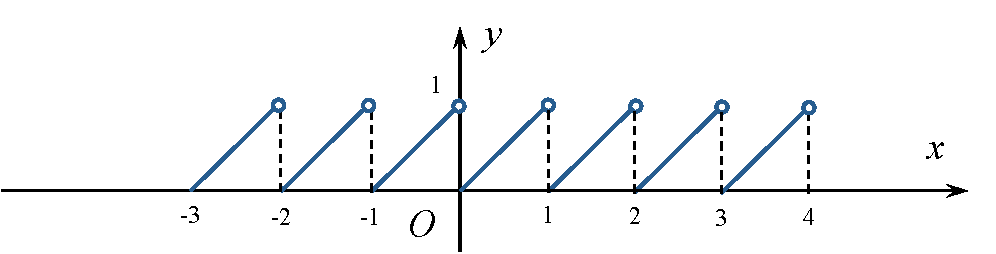
\includegraphics{./images/ch1/f1.pdf}}\quad $x-[x]$\\

	\resizebox{!}{2.5cm}{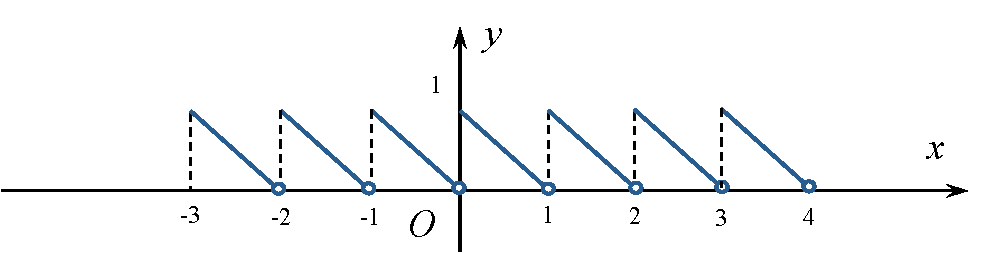
\includegraphics{./images/ch1/f2.pdf}}\quad $[x]-x+1$\\

	\resizebox{!}{2.5cm}{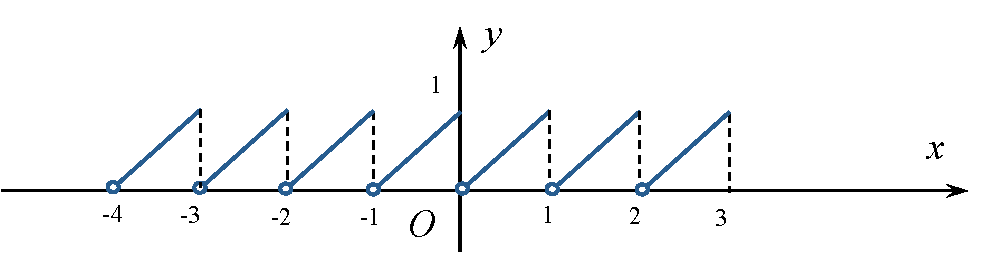
\includegraphics{./images/ch1/f3.pdf}}\quad $[-x]+x-1$
\end{center}
	
{\bf 例:}$(-1)^{[x]}$的图像?方波!

\subsubsection{\bf 【Dirichlet函数】}
  $$\bm{D}(x) =\left\{
  \begin{array}{ll}
  	1,\;& x\in\mathbb{Q} \\
  	0,\;& x\notin\mathbb{Q}
  \end{array}
  \right.$$
  \begin{itemize}
    \item $D(x)$在实数轴上处处无极限
	\item $D(x)$在实数轴上处处不连续
	\item {\b 仅在一点连续的函数:}$xD(x)$
  \end{itemize}

\subsubsection{\bf 【Riemann函数】*:} 

$(x\in[0,1])$
  $$\bm{R}(x) =\left\{
	\begin{array}{ll}
	1,\;&x=0\\
	\displaystyle\frac 1q,\;&x=\displaystyle\frac pq,\,p,q\mbox{互素}\\
	0,\;&x\notin\mathbb{Q}
	\end{array}
  \right. $$
  \begin{itemize}
    \item 对任意$x_0\in[0,1]$, $\lim\limits_{x\to x_0}R(x)=0$
    \vspace{1ex}
    \item $R(x)$在{\b 无理数点连续, 有理数点不连续}
  \end{itemize}

\subsubsection{【初等函数】}

\begin{enumerate}
  \item {\bf 幂函数:} $y=x^a,\; (a\in\mathbb{R})$
  \item {\bf 指数函数:} $y=a^x,\; (a>0,a\ne 1)$
  \begin{itemize}
    \item {\b $y=e^x$}
  \end{itemize}
  \item {\bf 对数函数:} $y=\log_ax,\; (a>0,a\ne 1)$
  \begin{itemize}
    \item {\b$y=\ln x$}
  \end{itemize}
  \item {\bf 三角函数:} $\sin x, \,\cos x,\, \tan x, \,\cot
  x,\, \sec x,\, \csc x$
  \item {\bf 反三角函数:} $\arcsin x, \,\arccos x, \arctan x,
  \ldots$
\end{enumerate}
{\bf{要求:}} 熟练掌握初等函数的定义、性质和相互推导的公式


\subsubsection{【($n$)次多项式(函数)】}

  $$P_n(x)=\sum_{i=0}^na_ix^i,
  \;(a_i\in\mathbb{R},i=1,2,\ldots,n)$$
  \begin{itemize}
    \item { $n$次多项式方程$P_n(x)=0$在$\mathbb{R}$上最多有$n$个根 (包含重根) ,在
    $\mathbb{C}$上有且仅有$n$个根(包含重根)}
    \item { 设$x_i\in\mathbb{C}(i=1,2,\ldots,n)$为$P_n(x)=0$的全部根 ,则
    $$P_n(x)=a_n\prod_{i=1}^n(x-x_i)$$}
    \item { 已知$P_n(x)$在$n+1$个点处的值, 可以唯一确定$P_n(x)$}
  \end{itemize}

\subsubsection{【有理函数】}

$$f(x)=\frac{P(x)}{Q(x)}, \quad\mbox{其中}P(x),Q(x)\mbox{均为多项式函数}$$
  
{\bf 注:}任意有理函数总可以化为一个多项式函数和一个真有理函数(分子的次数比分母低)的和
	  
{{\bf 例:}用多项式除法化简以下函数}
$$\frac{5x^3+3x^2+1}{x+1}$$

\subsubsection{【双曲函数】}

{\small $$\sinh x =\df{e^x-e^{-x}}{2}, \quad
\cosh x =\df{e^x+e^{-x}}{2}, \quad\tanh x=\df{\sinh
x}{\cosh x}, \ldots$$}

\section{曲线的参数方程和极坐标方程}

{\bf 问题:}$y=f(x)$能否表示平面上的所有曲线?
	
{\bf 或者:}怎样才能更好地表示平面上的曲线?\ps{例如:$x^2+y^2=1,xy=1,x=y^2,\ldots$}

\begin{shaded}
	\begin{center}
		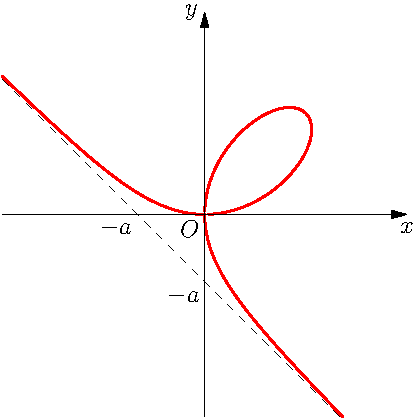
\includegraphics[width=5.5cm]{./images/ch1/dicartesCurve.pdf}

		{\bf Descartes叶形线}
	\end{center}
	\bigskip
	\begin{itemize}
	  \item {\bf 参数方程:}
	  	$$\left\{\begin{array}{l}
	  		x=\df{3at}{1+t^3},\\[1em] y=\df{3at^2}{1+t^3}
	  	\end{array}\right.\;(t\in\mathbb{R})$$
	  	\vspace{-1em}
	  \item {\bf 隐函数方程:}
	  	$$x^3+y^3-3axy=0$$
	\end{itemize}
\end{shaded}

{\bf 例:}求过平面上两点$P_i(x_i,y_i)\,(i=1,2)$的直线方程
		  
$$k=\df{y_2-y_1}{x_2-x_1}=\df{y_2-y_1}{x_2-x_1}$$
由此可给出直线的平面直角方程。若参数化
$$\df{y_2-y_1}{y_2-y_1}=\df{x_2-x_1}{x_2-x_1}=t$$
则有
$$y=ty_2+(1-t)y_1,\quad x=tx_2+(1-t)x_1,\quad (t\in\mathbb{R})$$
		  
{\bf 注:}
\begin{itemize}
  \item 参数方程必须标明参数的取值范围!!!
  \item {利用参数方程可以表示平面上的任意曲线}
  \item {任意曲线的参数方程均不唯一}
\end{itemize}

\subsubsection{【极坐标】}

$$(x,y)\;\to\;(\rho\cos\theta,\rho\sin\theta)\quad
(\rho>0,\theta\in\mathbb{R})$$
	
{{\bf 例:}求以下曲线的极坐标方程\hfill P38-例9}
		
\begin{enumerate}
  \item $y=kx,(k\in\mathbb{R})$
  \item $x+y=1$
  \item $x^2+y^2=R^2,\,(R>0)$
  \item $(x^2+y^2)^2=2a^2xy$
\end{enumerate}
	
{\bf 思考:}将极坐标方程化为平面直角方程应注意些什么?

\vspace{4em}

{\bf 【课堂练习与思考题】}

\begin{itemize}
  \item 习题1.1:(C)应用题
  \item 习题1.2:3,17
  \item 习题1.3:6
\end{itemize}

{\bf 【课后作业】}
	
\begin{itemize}
  \item 习题1.1:4(2),10
  \item 给出P9例6中二维球极投影映射中:
  
  (1)$Q$的极坐标与$P$的横坐标的对应关系;
  
  (2)$Q$的坐标与$P$的坐标的对应关系;
  
  (3)描述如何将一个单位球面映射为一个二维平面,给出相应的坐标对应关系。
  \item 习题1.2:8,12,13,21
  \item 给出P23例14中的三角波的函数表达式
  \item 习题1.3:5
\end{itemize}